% =====================================================================
%  IF4070 Milestone 1 Part 1 — kerangka laporan
%
%  Ini KERANGKA, bukan laporan. Semua isi analisis, aksioma, keputusan
%  pemodelan, dan pembahasan ditulis tangan: spek halaman 5 melarang
%  AI generatif untuk bagian-bagian itu.
%
%  Build:  make report      (menghasilkan laporan/laporan.pdf + hitung halaman)
%
%  Notasi DL boleh diketik langsung sebagai unicode (⊑ ∃ ⊓ ≡ ¬ ≥ ⊥ ⊤ ∘).
%  tools/build_report.py menerjemahkannya ke perintah LaTeX sebelum compile.
% =====================================================================
\documentclass[11pt,a4paper]{article}

\usepackage[T1]{fontenc}
\usepackage[utf8]{inputenc}
\usepackage[indonesian]{babel}
\usepackage[margin=2.5cm,top=2.5cm,bottom=2.5cm]{geometry}
\usepackage{amsmath,amssymb}
\usepackage{graphicx}
\usepackage{booktabs}
\usepackage{longtable}
\usepackage{array}
\usepackage{tabularx}
\usepackage{xcolor}
\usepackage{caption}
\usepackage{enumitem}
\usepackage{titlesec}
\usepackage{fancyhdr}
\usepackage[hidelinks]{hyperref}
\usepackage{microtype}

\graphicspath{{gambar/}}

\definecolor{todofg}{HTML}{B35C00}
% inline, aman dipakai di dalam sel tabel (tidak memancarkan \par)
\newcommand{\todo}[1]{\textcolor{todofg}{\textbf{[TODO}\ifx\relax#1\relax\else\textbf{:}\enspace #1\fi\textbf{]}}}

\setlength{\parskip}{4pt}
\setlength{\parindent}{0pt}
\renewcommand{\arraystretch}{1.15}

\newcommand{\grup}{K11}   % harus sama dengan config.yaml

\pagestyle{fancy}
\fancyhf{}
\fancyhead[L]{\small IF4070 M1P1}
\fancyhead[R]{\small Kelompok \grup}
\fancyfoot[C]{\small\thepage}
\renewcommand{\headrulewidth}{0.4pt}

\title{\textbf{Tugas Besar IF4070\\Representasi Pengetahuan dan Penalaran}\\[6pt]
       \large Milestone 1 Part 1\\Daftar Aturan, Competency Question, dan Ontologi}
\author{Kelompok \grup}
\date{29 Oktober 2026}

\begin{document}

% =====================================================================
% COVER
% =====================================================================
\begin{titlepage}
\centering
\vspace*{2cm}
{\Large\bfseries Tugas Besar IF4070\\ Representasi Pengetahuan dan Penalaran\par}
\vspace{1.2cm}
{\LARGE\bfseries Milestone 1 Part 1\par}
\vspace{0.4cm}
{\large Daftar Aturan, \emph{Competency Question}, dan Ontologi OWL\par}
\vspace{2cm}

\begin{tabular}{ll}
\toprule
\textbf{Kelompok} & \grup \\
\textbf{Domain}   & Kartu \emph{bridge} (\emph{contract bridge}) \\
\bottomrule
\end{tabular}

\vspace{1.5cm}
\begin{tabular}{lll}
\toprule
\textbf{Nama} & \textbf{NIM} & \textbf{Tanggung jawab} \\
\midrule
Ahmad Ibrahim & 13523089 & \todo{} \\
Bintang Hijriawan Jachja & 13521003 & \todo{} \\
Michael Alexander Angkawijaya & 13523102 & \todo{} \\
\bottomrule
\end{tabular}

\vfill
{\small Program Studi Teknik Informatika\\
Sekolah Teknik Elektro dan Informatika\\
Institut Teknologi Bandung\\[4pt]
2026\par}
\end{titlepage}

% =====================================================================
\section{Deskripsi Domain}
% =====================================================================

\todo{Tulis bagian ini tangan.}
\textbf{Batasan domain:} apa yang masuk dan apa yang sengaja dikeluarkan, sebutkan
cakupan \emph{scope} secara eksplisit (level detail, periode aturan, entitas yang
diabaikan).

\textbf{Sumber:} daftar dokumen di folder \texttt{sumber/} beserta apa yang diambil
dari masing-masing.

\textbf{Perbedaan struktural dari domain terdekat yang dilarang:}
spek mewajibkan \emph{satu paragraf} yang menjelaskan kenapa domain ini tidak
serumpun dengan domain di daftar larangan. Sebut domain terdekatnya, lalu
tunjuk perbedaan struktur konsepnya — bukan perbedaan nama atau tema.

% =====================================================================
\section{Aksioma Inti}
% =====================================================================

Minimal 10 aksioma dalam notasi logika deskripsi formal, masing-masing dengan
ID aturan yang diwakili dan alasan pemilihan konstruksinya.

\begin{longtable}{@{}p{0.6cm} p{6.6cm} p{1.5cm} p{4.2cm}@{}}
\toprule
\textbf{ID} & \textbf{Aksioma} & \textbf{Aturan} & \textbf{Alasan konstruksi} \\
\midrule
\endfirsthead
\toprule
\textbf{ID} & \textbf{Aksioma} & \textbf{Aturan} & \textbf{Alasan konstruksi} \\
\midrule
\endhead

% contoh bentuk baris — hapus dan ganti dengan aksioma kelompok:
% A1 & $X \sqsubseteq \exists r.Y$ & R1 & ... \\
\midrule
\bottomrule
\end{longtable}

\todo{Isi tabel di atas. Alasan konstruksi harus menjelaskan kenapa ∃/∀/⊓/
kardinalitas/disjointness dipilih, bukan sekadar mengulang bunyi aksioma.}

% =====================================================================
\section{Pemenuhan Fitur Wajib}
% =====================================================================

\begin{longtable}{@{}p{4.6cm} p{5.8cm} p{3.4cm}@{}}
\toprule
\textbf{Fitur wajib} & \textbf{Aksioma yang memakai} & \textbf{CQ yang bergantung} \\
\midrule
\endfirsthead
\toprule
\textbf{Fitur wajib} & \textbf{Aksioma yang memakai} & \textbf{CQ yang bergantung} \\
\midrule
\endhead
Kelas terdefinisi yang menghasilkan klasifikasi terinferensi & & \\
Restriksi tipe data atau kardinalitas & & \\
Properti transitif / invers / rantai properti & & \\
Disjointness & & \\
\midrule
\bottomrule
\end{longtable}

\todo{Setiap fitur wajib harus dipakai minimal satu CQ. Fitur yang hanya
ditempelkan tanpa CQ tidak dihitung.}

% =====================================================================
\section{Jawaban \emph{Competency Question}}
% =====================================================================

Untuk setiap CQ: kueri DL Query yang dijalankan di Protégé, hasilnya, dan jalur
penalarannya.

\todo{Ulangi blok berikut untuk setiap CQ1..CQn.}

\subsection*{CQ1}
\begin{tabular}{@{}p{2.2cm} p{11.3cm}@{}}
\textbf{Pertanyaan} & \todo{} \\
\textbf{DL Query} & \texttt{\todo{ekspresi DL Query yang diketik di tab DL Query}} \\
\textbf{Hasil} & \todo{isi hasil beserta jumlah individu/kelas} \\
\textbf{Jalur penalaran} & \todo{aturan mana yang berperan, dalam urutan apa} \\
\end{tabular}

\todo{Minimal dua CQ harus berjawaban "Tidak" dan dijelaskan mengapa tidak.}

% =====================================================================
\section{Studi Kasus Inkonsistensi}
% =====================================================================

\begin{enumerate}[leftmargin=*]
  \item \textbf{Kontradiksi yang disuntikkan:} \todo{apa yang diubah di salinan
        \texttt{\_inkonsisten.owl} dan kenapa itu menghasilkan inkonsistensi}
  \item \textbf{Penjelasan dari Protégé:} lihat gambar di bawah.
  \item \textbf{Cara membaca penjelasan:} \todo{urai rantai aksioma yang dilaporkan
        reasoner, dari premis sampai ⊥}
  \item \textbf{Cara memperbaiki:} \todo{perbaikan mana yang dipilih dan kenapa
        itu yang benar secara model, bukan sekadar yang menghilangkan galat}
\end{enumerate}

\begin{figure}[h]
\centering
% 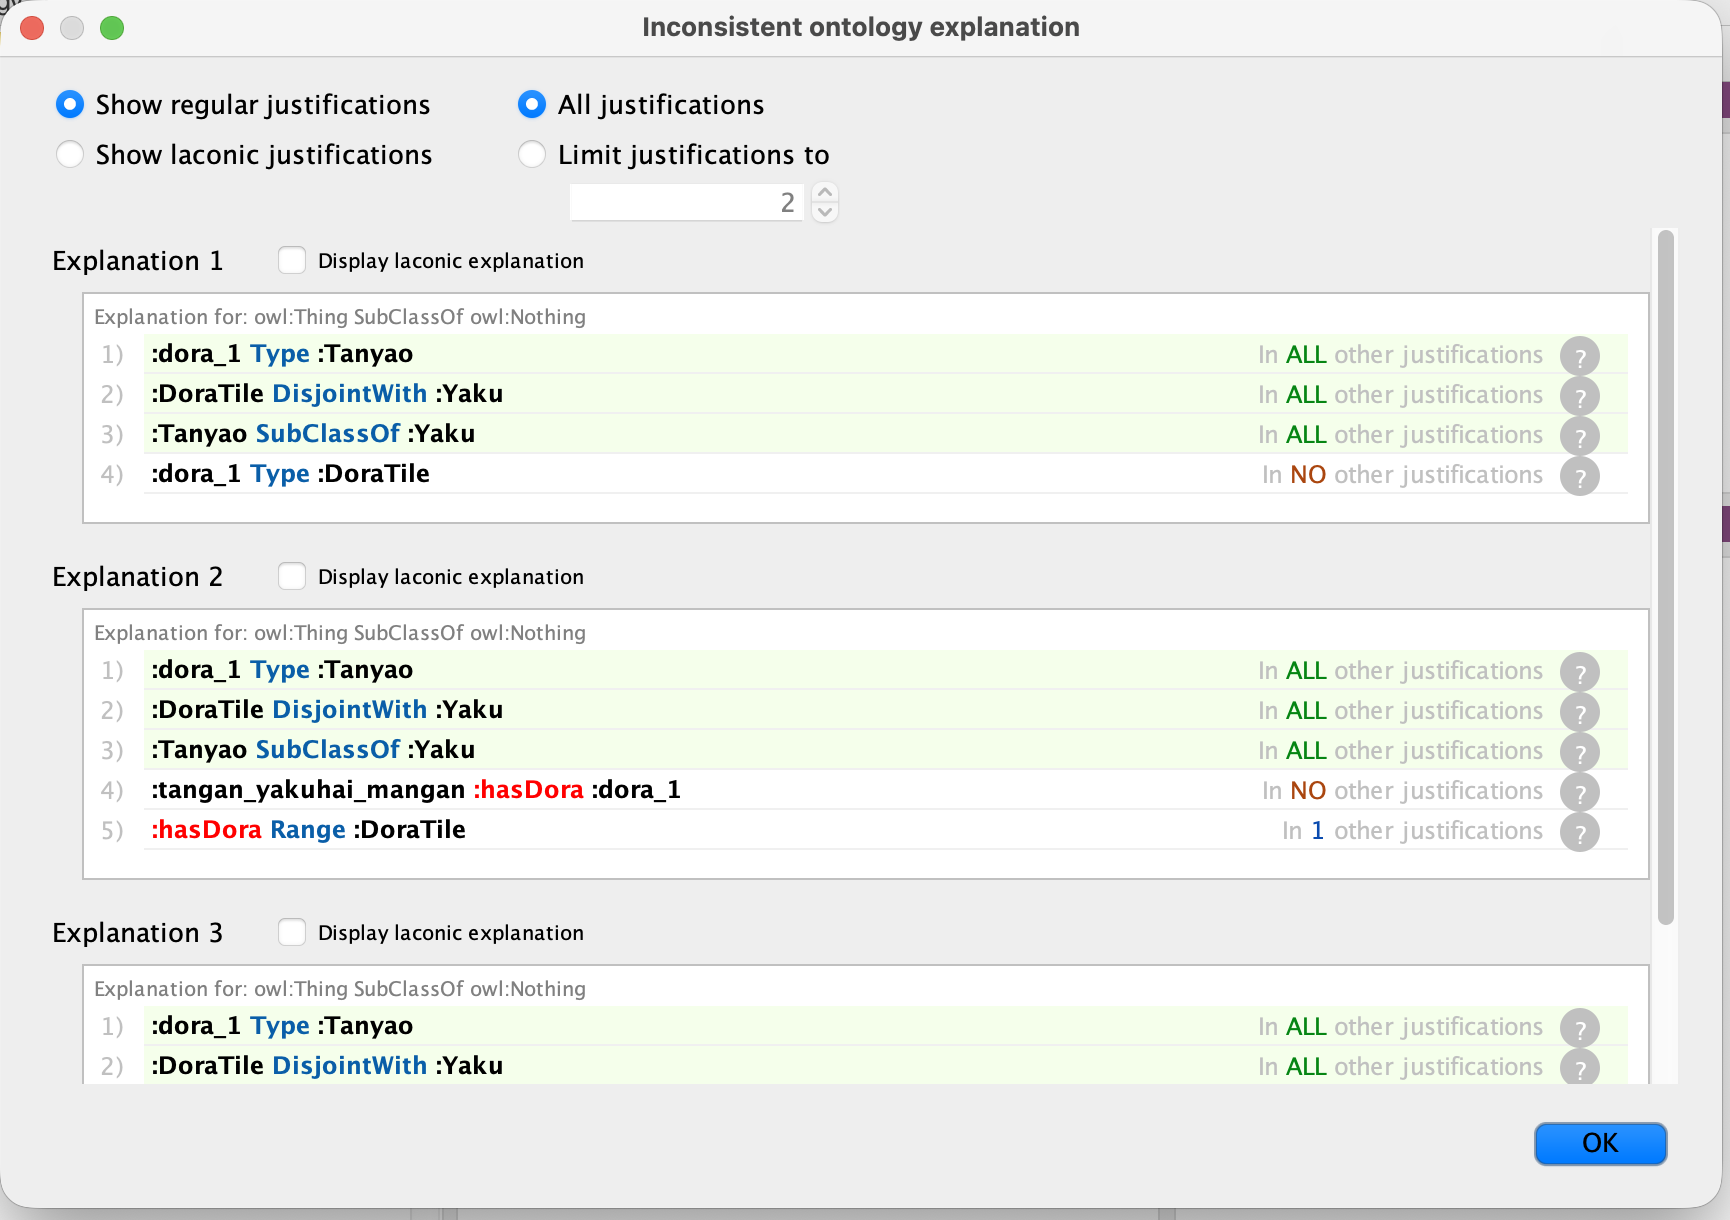
\includegraphics[width=0.9\linewidth]{penjelasan_inkonsisten.png}
\fbox{\parbox[c][5cm][c]{0.85\linewidth}{\centering
\todo{screenshot jendela \emph{Explain inconsistency} di Protégé}\\[4pt]
\small bukti ini wajib berupa gambar, tidak bisa diganti teks}}
\caption{Penjelasan inkonsistensi dari HermiT di Protégé.}
\end{figure}

% =====================================================================
\section{Keputusan Pemodelan}
% =====================================================================

Minimal tiga keputusan. Untuk masing-masing: alternatif yang dipertimbangkan dan
alasan alternatif itu tidak dipilih.

\todo{Ulangi pola berikut tiga kali atau lebih.}

\textbf{Keputusan 1:} \todo{keputusan}\\
\textit{Alternatif yang dipertimbangkan:} \todo{}\\
\textit{Alasan tidak dipilih:} \todo{}

% =====================================================================
\section{Aturan Non-OWL}
% =====================================================================

\todo{Untuk setiap aturan bertanda non-OWL di daftar aturan, tulis alasan
teknisnya: agregasi yang tidak dimiliki OWL, sifat monoton logika deskripsi,
atau kebutuhan asumsi dunia tertutup. Sebutkan juga rencana implementasinya di
Part 2 (Prolog).}

\begin{longtable}{@{}p{1.2cm} p{5.4cm} p{6.3cm}@{}}
\toprule
\textbf{Aturan} & \textbf{Bunyi aturan} & \textbf{Alasan teknis tidak bisa di OWL} \\
\midrule
\endfirsthead
\toprule
\textbf{Aturan} & \textbf{Bunyi aturan} & \textbf{Alasan teknis tidak bisa di OWL} \\
\midrule
\endhead
\midrule
\bottomrule
\end{longtable}

% =====================================================================
\section{Pembagian Tanggung Jawab}
% =====================================================================

\begin{tabular}{@{}p{3.4cm} p{2.4cm} p{8.2cm}@{}}
\toprule
\textbf{Anggota} & \textbf{NIM} & \textbf{Tanggung jawab} \\
\midrule
 & & \\
 & & \\
 & & \\
\bottomrule
\end{tabular}

% =====================================================================
\section{Log Penggunaan AI}
% =====================================================================

Wajib jujur. Penggunaan yang tidak dideklarasikan membuat bagian terkait bernilai nol.

\begin{longtable}{@{}p{2.3cm} p{3.6cm} p{3.4cm} p{4.2cm}@{}}
\toprule
\textbf{Kakas} & \textbf{Tujuan penggunaan} & \textbf{Bagian yang terpengaruh} & \textbf{Cara kelompok memeriksa} \\
\midrule
\endfirsthead
\toprule
\textbf{Kakas} & \textbf{Tujuan penggunaan} & \textbf{Bagian yang terpengaruh} & \textbf{Cara kelompok memeriksa} \\
\midrule
\endhead
\midrule
\bottomrule
\end{longtable}

% =====================================================================
\section*{Referensi}
\addcontentsline{toc}{section}{Referensi}
% =====================================================================

\begin{thebibliography}{9}
\bibitem{dlhandbook} Baader, F., Calvanese, D., McGuinness, D., Nardi, D., dan
  Patel-Schneider, P. (2007). \emph{The Description Logic Handbook}.
\bibitem{gruninger} Grüninger, M. dan Fox, M. S. (1995). Methodology for the Design
  and Evaluation of Ontologies. \emph{Workshop on Basic Ontological Issues in
  Knowledge Sharing, IJCAI-95}.
\bibitem{protege} Dokumentasi Protégé dan Protégé Wiki, panduan pengguna dan
  tutorial OWL.
\end{thebibliography}

\todo{Tambahkan referensi dokumen sumber domain (S1, S2, ...) dengan penulis,
tahun, dan cara aksesnya.}

% =====================================================================
\clearpage
\appendix
\section{Lampiran: Daftar Aturan Versi Final}
\label{sec:lampiran}
% =====================================================================

Tabel ini dihasilkan otomatis dari \texttt{aturan/daftar-aturan.md} saat
\texttt{make report}, jadi selalu sinkron dengan versi yang dibekukan.

\input{generated/daftar-aturan}

\end{document}
